%----------------------------------------------------------------------------
\chapter{System Overview}

In this chapter, I overview the complete system. I explain the main design decisions, and some more exciting implementation details.

\section{ALPR pipeline}

The applied pipeline is shown by Figure \ref{fig:pipeline}. It compresses the traditional tasks into as few steps as possible. The structure is like the one used in WPOD-NET\cite{WPOD-NET}, with some differences. First, a RetinaNet\cite{RetinaNet} detector is used for both vehicle and plate localization (instead of a YOLOv2\cite{YOLOv2} vehicle-only detector). The rectification step is excluded from our pipeline, which is a drawback in plate image quality. However, WPOD-NET's rectification supports only one plate scale, so adding it would not be a general solution, in our opinion. On the other hand, it would increase the computational load as it must run separately for each detected vehicle. The second step is to filter possible plate objects based on location and confidence scores. The third is to cut plate objects from the original image.

\begin{figure}[H]
 \centerline{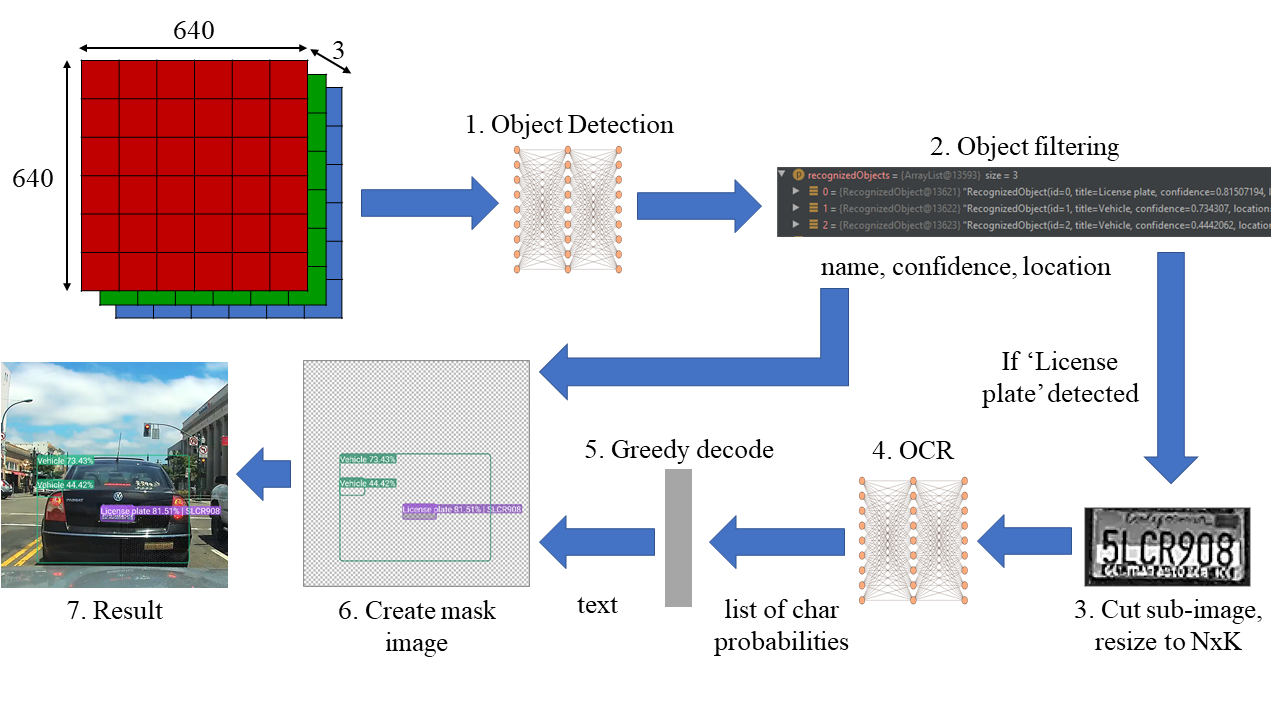
\includegraphics[width=1.0\columnwidth]{.//Figure/System/pipeline.png}}
 \caption{The applied ALPR pipeline.}
 \label{fig:pipeline}
\end{figure}

The pipeline models are dynamically quantized TensorFlow Lite converted networks. On a Samsung Galaxy S10 smartphone, where an image contains only one license plate, the average runtime is roughly 160 ms. The processing steps are as follows:

\begin{itemize}
  \item image preprocessing (9 ms)
  \item detector inference (75 ms on GPU)
  \item cutting and resizing the license plate image segment (3 ms)
  \item OCR inference (37 ms on CPU)
  \item Greedy decoding (<1 ms)
  \item creating mask image (33 ms)
\end{itemize}

This runtime may change depending on the number of plates on a picture, as the OCR steps must be repeated on each license plate image segment.

Table \ref{tab:OCR_model_runtimes} summarizes the runtimes of different OCR models. Besides the best-performing network, I also tested the initial architecture (batch 128). It runs in 37 ms on the device's GPU. Keeping in mind the runtime, it is worth sacrificing marginal quality (+\({9.5} \times {10^{-3}}\) loss) to acquire a $1.5\times$ speed-up. As a reference, Google's MLKit Vision Text Recognizer\cite{MLKitTextRecognition} runs in 40 ms on the same plate image with a single line of text. The MLKit model is a multiblock recognizer. However, when more than one block is present, its runtime increases drastically.

\begin{table}[htb]
\caption{Running time in milliseconds for OCR models.}
\label{tab:OCR_model_runtimes}
\noindent
\centering
\begin{tabular*}
{\columnwidth}{@{\extracolsep{\stretch{1}}}*{6}{r}@{}}
    model & host & input & size [KB] & loss & inference [ms]\\ \hline
    batch 128 & CPU & 50x500x3 & $639$ & $0.0848$ & $37$ \\
    MLKit & CPU & 50x500x3 & $?$ & $?$ & $40$ \\
    batch 128 & GPU & 50x500x3 & $639$ & $0.0848$ & $50$ \\
    Hyper1st & CPU & 50x500x3 & $4,447$ & $0.0753$ & $56$ \\
    MLKit & CPU & 200x200x3 & $?$ & $?$ & $72$ \\
    Unfolding & CPU & 200x200x3 & $3,133$ & $0.0991$ & $221$ \\
    Unfolding & GPU & 200x200x3 & $3,133$ & $0.0991$ & $372$ \\
\end{tabular*}
\end{table}

\section{Frontend}

The client application's main task is to detect stolen vehicles, then report them using location and time data. The application runs the pipeline on the device, and it is possible to run an evaluation on loaded images and the live image feed. The user constantly sees what has been recognized. Stolen vehicle and user data are stored in a local SQLite database, synchronized in the background with the API. Available camera operations include front/back camera switching, image saving, tap to focus, and pinch to zoom. I present the Android application's architecture and some details in the following.

The application can receive inputs from two different sources. The first option is to load an image from the storage. In this case, the image is processed only once, and the meta-information (GPS location, UTC timestamp) is extracted from the image's Exif (Exchangeable image file format) content. This format is supported by almost any type of smartphone (if not, fallback values are used, which cannot be reported to the server). This is important because otherwise, a stolen vehicle image from the past could overwrite a more recent recognition on the server when reporting the match. The other option is to process the live camera feed. For this, the current camera frame is fed into the pipeline. When the results are ready, the current live frame is processed, meaning that frames are discarded while the pipeline is processing. The live feed results are accompanied by the device's location and system UTC timestamp information. If they are unavailable, fallback values are used. In both cases, image preprocessing steps are applied shown by Figure \ref{fig:image_preprocessing}. Some images of the application are shown in Figure \ref{fig:AppImages}.

\begin{figure}[htb]
 \centerline{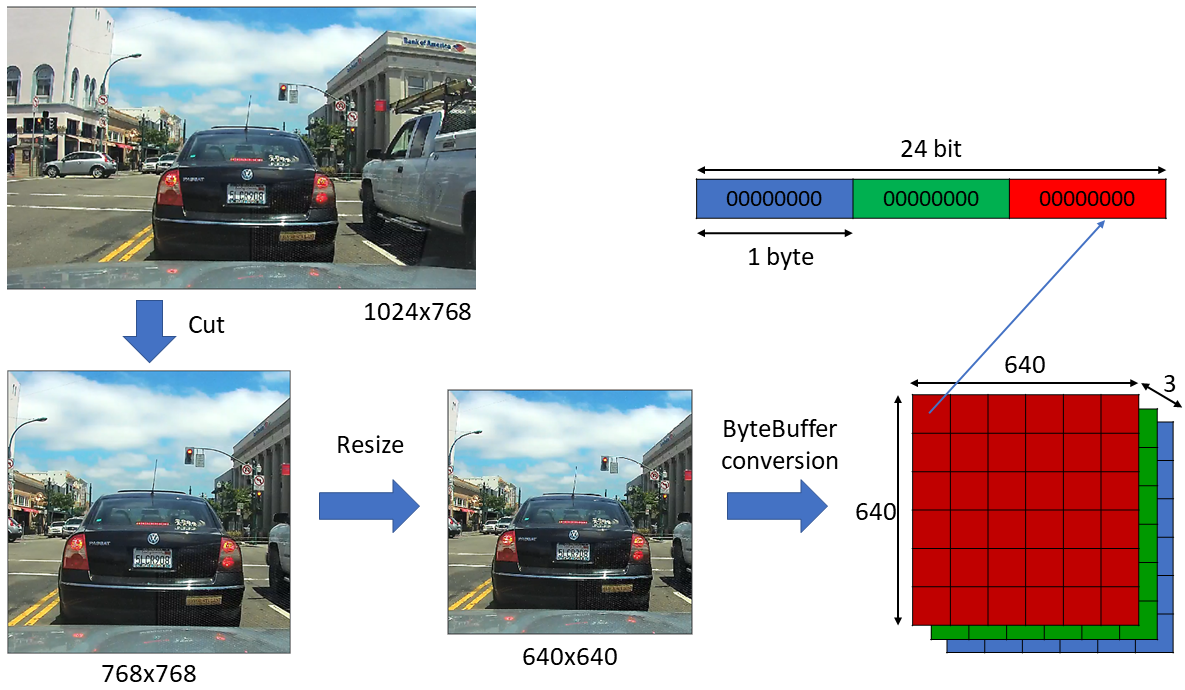
\includegraphics[width=0.9\columnwidth]{.//Figure/System/image_preprocessing.png}}
 \caption{Image preprocessing steps before feeding the pipeline.}
 \label{fig:image_preprocessing}
\end{figure}

\begin{figure}[H]
 \centerline{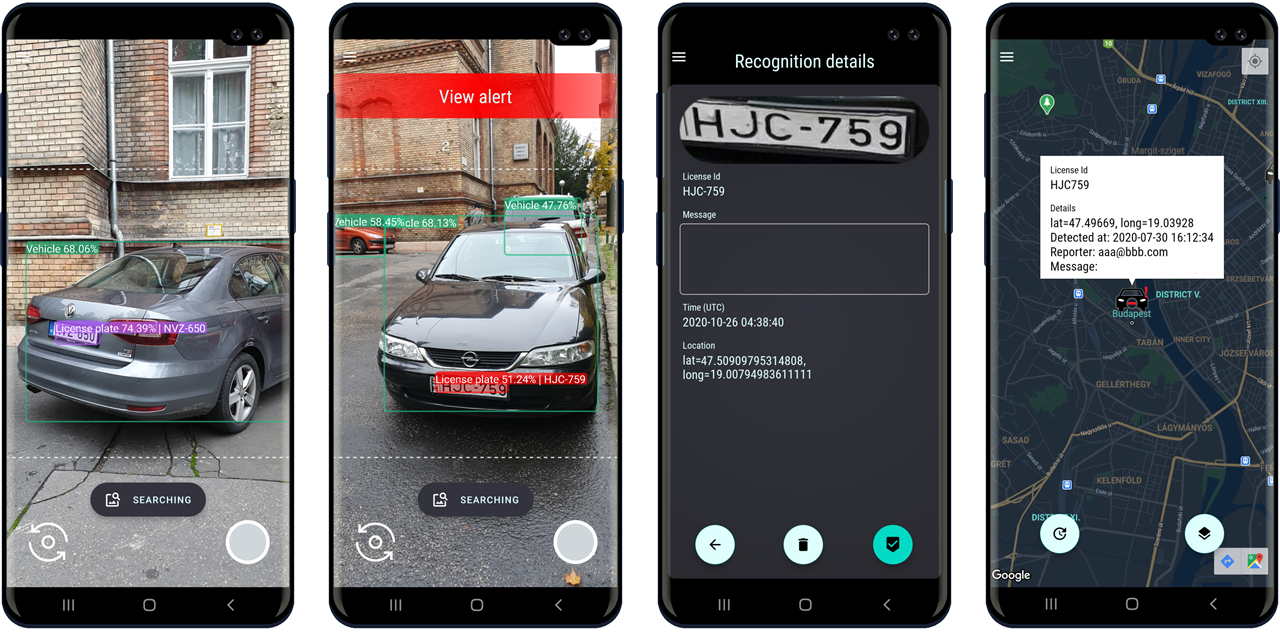
\includegraphics[width=1.0\columnwidth]{.//Figure/System/AppImages.png}}
 \caption{Live feed recognition (1st screen) and an identified stolen vehicle (2nd screen). Details can be inspected and a message can be added to a recognition (3rd screen). When a vehicle is reported, its last known position is visible on the map (4th screen).}
 \label{fig:AppImages}
\end{figure}

\subsection{Architecture}

I used the \textit{Model View ViewModel} (MVVM) UI design pattern. It is an event-driven model invented by Microsoft to take advantage of data binding capabilities. In MVVM, the View contains UI descriptive code often in a declarative (XML, XAML, HTML) form, and the connection to the ViewModel is realized with explicit data binding. Therefore, there are fewer classic coding tasks in Views, and the business logic components can be easily separated.

There are sub-layers in the model level of the application. I explain the hierarchy through the steps of reporting a single item. Suppose a new stolen vehicle was detected on the live camera feed, and the user selected to report it. In this case, the user sees a ReportActivity, which has a ViewModel storing the UI state. The report item gets stored in a list wrapped in a LiveData object (observable from the Activity). When the user clicks on the send button, the related data is transmitted to the RepositoryService in the model layer. Inside this service, there is the ReportRepository. It hides further data operations (database handling, API communication) from the outside. When it receives a new report, it transforms it into a format stored in the Report table and persists with ReportDAO (data access object) to the database. After that, it calls ApiService to send the report to the server. When the response arrives from the API, ReportRepository updates the corresponding item in the database. Until the operation is unsuccessful, the user sees the report as pending. Pending items can be deleted or re-sent at any time. Figure \ref{fig:AndroidArchitecture} shows a high-level overview of the sub-layers and modules.

\begin{figure}[htb]
 \centerline{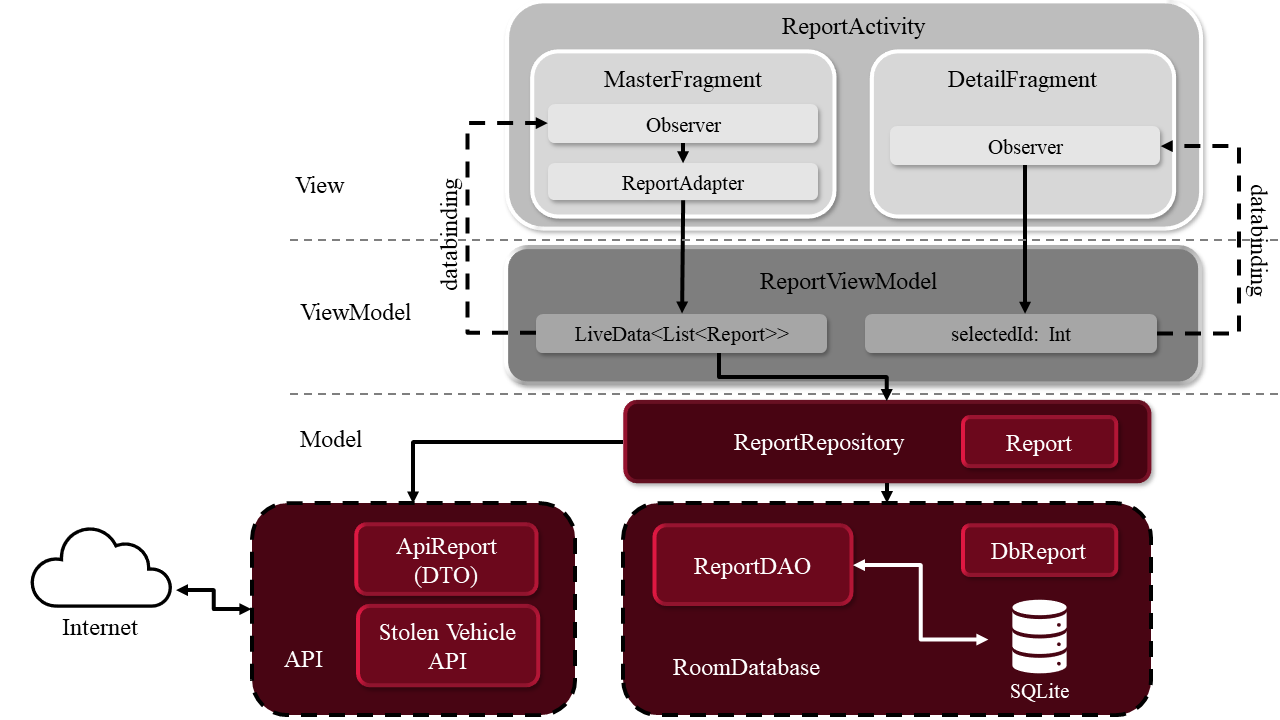
\includegraphics[width=1.0\columnwidth]{.//Figure/System/AndroidArchitecture.png}}
 \caption{MVVM layers in the application.}
 \label{fig:AndroidArchitecture}
\end{figure}

\newpage
\subsection{Database}

Beyond reports, the application stores several other information in its local relational database (list of stolen vehicles, account information, metadata). Outside the relational database, the application stores user preferences as key-value pairs. The complete database schema can be seen on Figure \ref{fig:AppData}. The persisted data schema differs from the in-memory data representation in order to be independent of higher-level modules. The schema of the data transfer objects (DTOs) is different for the same reason. This way, in case of API- or database schema changing, only the corresponding module needs to be updated, resulting in maintainable code.

\begin{figure}[H]
 \centerline{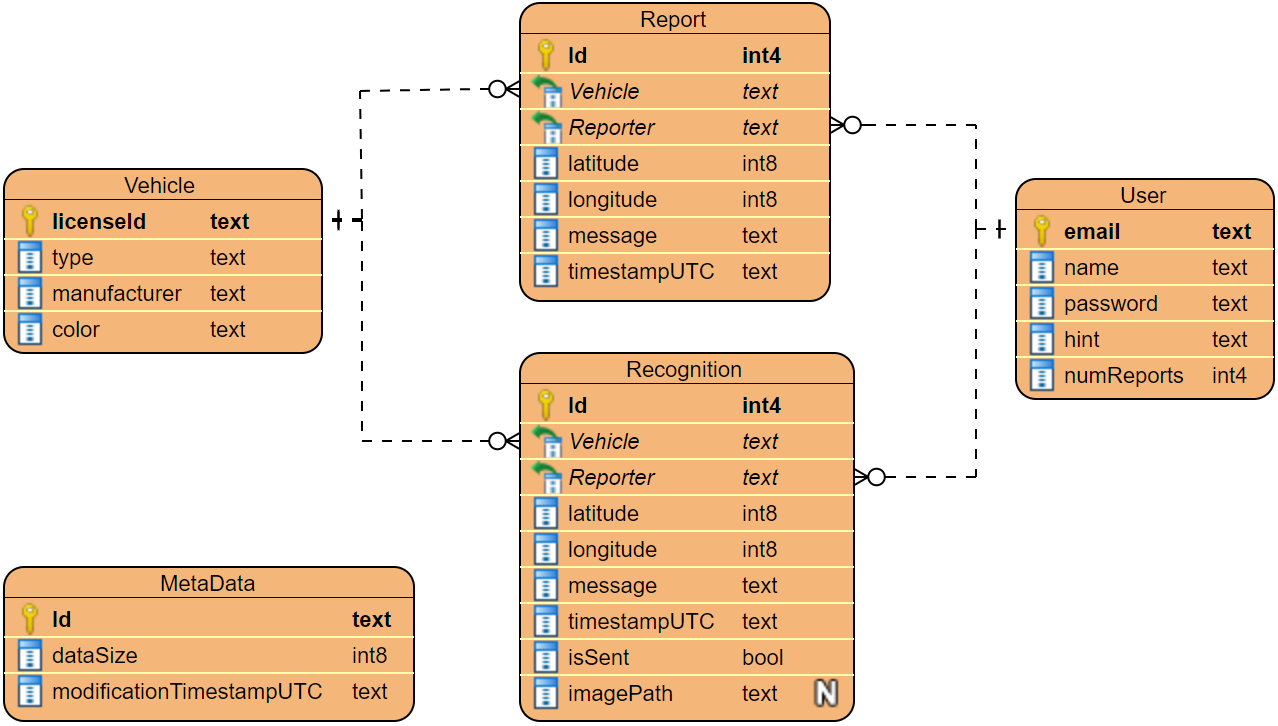
\includegraphics[width=1.0\columnwidth]{.//Figure/System/AppData.png}}
 \caption{Client application database schema.}
 \label{fig:AppData}
\end{figure}

\subsection{Vulnerabilities}

I would like to draw attention to some vulnerabilities of the application. By manipulating the Exif information of an image (changing coordinates, setting a timestamp to a later time), false recognition can be uploaded to the server, which can overwrite the current vehicle position record. Unfortunately, there is no robust solution to detect whether an image's Exif content has been modified or not by the time of this work. Also, an image editor can easily edit a recent photo (with valid Exif information) to contain a stolen vehicle in it. When using the live camera feed, pointing to an image of a stolen vehicle can also trigger a false report. These are opportunities for abuse due to the nature of image-based recognition. To prevent them, images inducing the report could also be uploaded to the server for further inspections. When a report's metadata is fallback or invalid, the application refuses to send them to the server.

\newpage
\section{Backend}

The server application provides the API for the clients and manages registered users. It has a stateless REST API, so a user needs to authenticate itself when querying the server.

\subsection{Architecture}

The server has a three-layered architecture (Figure \ref{fig:ServerStructure}). Because it is responsible for API service and data storage, it does not have a separate View layer (only a simple web-based UI is available). Instead of the UI layer, the communication layer through which the API services can be accessed. It is loosely coupled with other layers. User authentication is done with HTTP basic authentication. In the business logic layer, the Authenticator module checks requests and does not allow them to be executed when the required permissions are missing. The Interactor contains the main business logic. The data access layer contains the DAO classes responsible for handling their tables and providing a unified interface for retrieving/writing data.

\begin{figure}[htb]
 \centerline{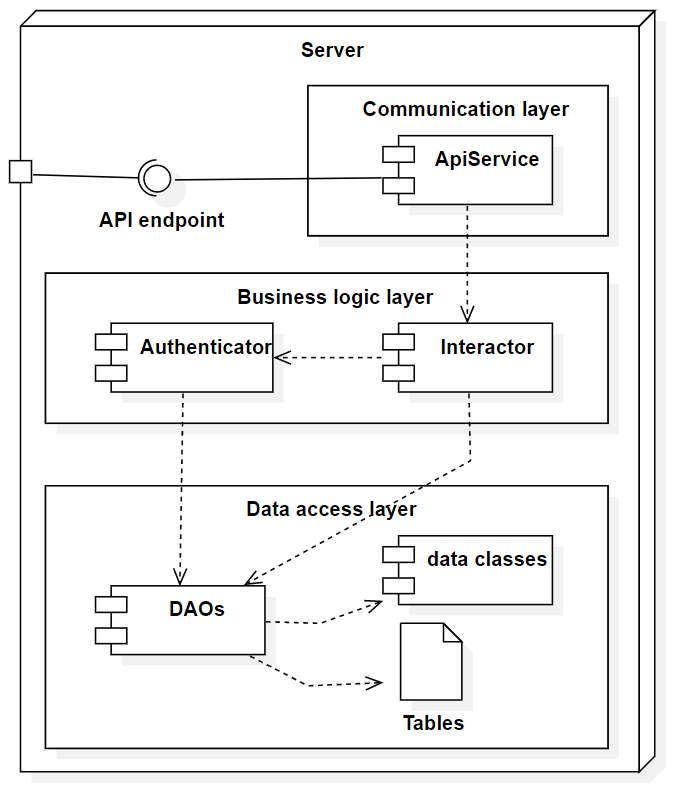
\includegraphics[width=0.5\columnwidth]{.//Figure/System/ServerStructure.png}}
 \caption{Structure diagram of the server.}
 \label{fig:ServerStructure}
\end{figure}

\subsection{Database}

Since I decided to use a self-created database, I briefly describe its main guidelines. It is a NoSQL variant with an in-memory approach. The tables store information in an object-oriented manner. The table contents are in JSON format (like in the case of MongoDB). The server uses the Gson library to encode and decode JSON files. Figure \ref{fig:ServerData} represents the schema of the stored objects.

There are tables of stolen vehicles, current reports, and user accounts. To these contents, history files(write only) are available. They store all items using a timestamp and a version number to support recovery and traceability. History tables are not stored in memory, and when a data table is updated, its corresponding history is automatically updated. There is a meta content storing size and timestamp information of the previous tables. Lastly, an Event table records system logs (also write-only).

The database serves requests from memory, making API responses fast because there is no need to wait for I/O operations. The memory content is synchronized with the corresponding table in the background. It is a viable solution as too many data records are never stored on the server (the images are not uploaded). I examined the most significant JSON object type (report) to validate this. One record takes up 173 bytes in the memory. The server needs 173 MB memory when 1 million records exist. It is a severe overestimation, though, as the stolen vehicles list obtained by web scraping typically has just a few thousand items (in the case of Hungary). That is the maximum number of records that the in-memory database ever has (when every stolen vehicle was detected). As the history content is stored persistently, extensive API usage neither saturates the memory. Given the scalability of the database, one server instance could handle all European countries.

\begin{figure}[htb]
 \centerline{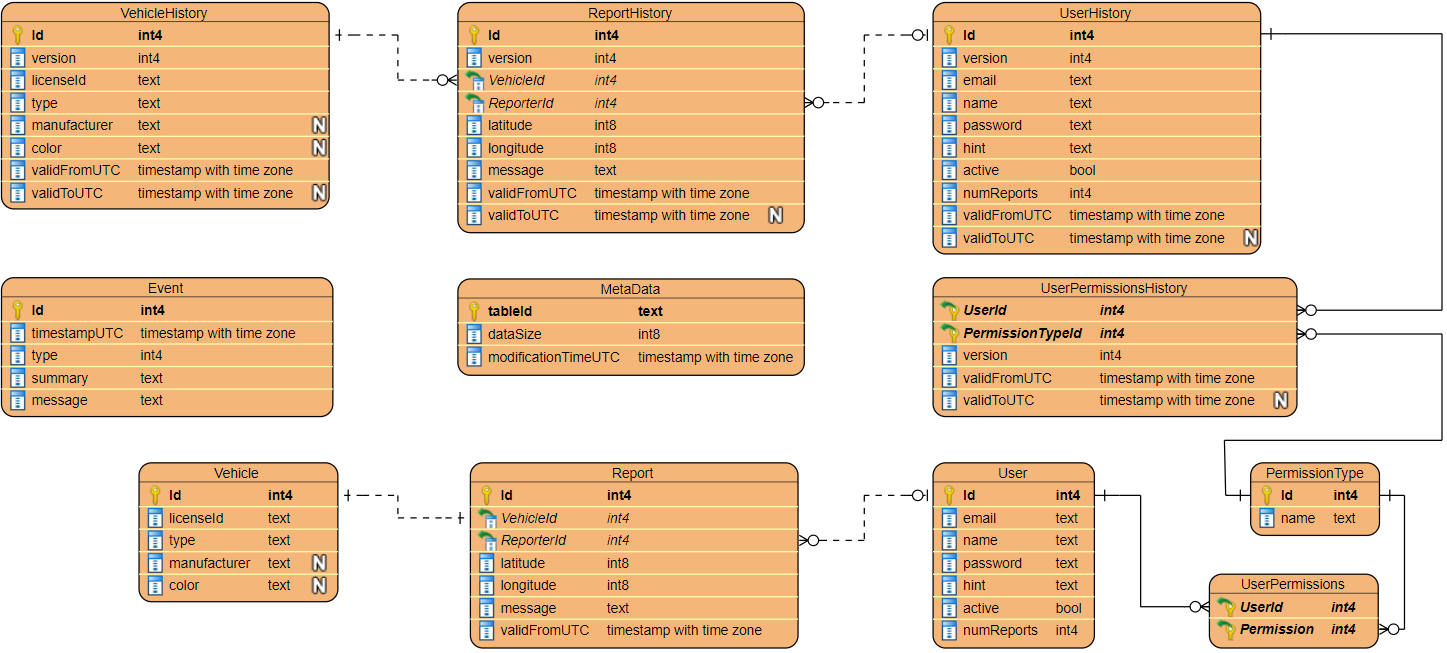
\includegraphics[width=1.0\columnwidth]{.//Figure/System/ServerData.png}}
 \caption{Server data schema.}
 \label{fig:ServerData}
\end{figure}

\subsection{API}

The API is divided into five parts: \textit{Vehicles, Reports, Report history, Self}, and \textit{Users}. These names are also the corresponding endpoint prefixes. All query endpoints have similar actions and a unified calling convention. All actions are subject to specific permissions, evaluated before serving. There is also a status page describing the API and its interface.

\subsection{Permission}

The nature of stored data (location and timestamp of stolen vehicles) could potentially allow abuses, so there is an allowlisting role-based permission model. Users with specific roles are eligible to execute various operations. There are ADMINISTRATOR, API\_REGISTER, SELF\_MODIFY, API\_GET, and API\_SEND permissions. Users can be uniquely identified by their inner server Id or email address.

\begin{itemize}
\item API\_GET lets an authorized account query report.
\item API\_SEND makes it possible to send recognitions to the server.
\item SELF\_MODIFY is needed to prevent blocklisted users from deleting themselves and re-register.
\item An ADMINISTRATOR user can modify the server and any user's permissions at any time. If someone's behavior is suspicious, an administrator can revoke permissions, delete a user, or deactivate and blocklist it. An administrator can also register a new user with specific permissions.
\item The default user (e.g., client application users) has an account with an API\_REGISTER role. This way, it is possible for newcomers to register their new accounts. If someone tries to use the application without signing in, this user is utilized. The only API permission is registration. Although someone can detect vehicles on-device, they cannot report them or see current reports. This API\_REGISTER role prevents anyone outside of the client application from registering. The default user can create a new account with SELF\_MODIFY, API\_GET, and API\_SEND permissions.
\end{itemize}

\subsection{Vulnerabilities}

The server stores sensitive data so attempts to abuse should be considered. Passwords are stored on the server in an encrypted format. No one can access user passwords - although administrators can block or delete users. Data access is based on an allowlisting model, meaning that anything which is not explicitly allowed is forbidden. The sensitive API endpoints (user actions, data uploads, and queries) are only available through HTTPS communication. Every database access is through predefined functions with a predefined list of allowed parameters, meaning that injection attacks are not possible. Users outside the client application cannot register, as the front-end contains a protected default user solely used to register new accounts. 

If the attacker is an inner user, its behavior can be monitored: if there are too many reports from the same account, or the report locations/timestamps are suspicious, administrators can revoke the API\_SEND permission or even block the user. When an account is blocked, it cannot query or upload. A blocked user cannot delete itself or re-register, meaning that it cannot access the server with the same email address anymore. If a badly-formatted report is received, the server discards it. If the report's metadata is invalid (non-existing GPS coordinates, future UTC timestamps), the server also discards it. If an attacker is an administrator, it can delete the current database state. However, the state can always be restored with the help of the history content, which cannot be deleted. Administrators cannot access other users' sensitive content (although they can delete accounts). Other administrators can block an administrator.